\frame
{
\frametitle{Reconocer la paradoja}
\vspace{1cm}
\begin{center}
	``El éxito es producto de rutinas arraigadas/
	las rutinas arraigadas destruyen la adaptabilidad''
\end{center}
\hspace{2cm}
\begin{columns}
\begin{column}{0.6\textwidth}
\end{column}
\begin{column}{0.4\textwidth}
	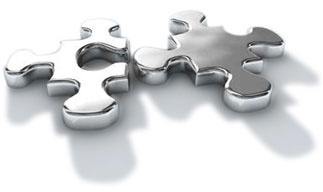
\includegraphics[width=0.9\textwidth]{img/adaptabilidad}
\end{column}
\end{columns}
}

\frame
{
\frametitle{Reconocer la paradoja}
\framesubtitle{Confesar la paradoja}
\begin{itemize}
	\item \emph{Organizational Ecology} % proponen leyes de seleccion natural y variacion aleatoria de la biologia se aplican tambien en la vida organizativa.
	\item La \blue{idea central} es si una empresa sigue adelante por lo que sea, suerte, cerebro, etc.
	\item Los ganadores se mantienen \blue{firmes} en sus rituales.
	\item La \blue{variación} es el enemigo de la \red{calidad}.
	\item \red{Trampa:} las rutinas del éxito de algunas empresas son la \blue{vulnerabilidad} mayor.
	\item Debemos crear una organización \blue{adaptable}, pero \red{cuidado}.
\end{itemize}
}

\frame
{
\frametitle{Reconocer la paradoja}
\framesubtitle{Busque los grande fallos}
\begin{itemize}
	\item Es \red{bueno} tener grandes \blue{fallos}, por que así \blue{aprendemos}.
	\begin{itemize}
		\item \emph{Si no se ha roto, no lo arregles.}
		\item \emph{Si no se ha roto, arreglalo de todos modos.}
		\item \emph{Si no se ha roto, es que no has mirado bien.}
	\end{itemize}
	\item \emph{AT\&T} y \emph{Apple} han fallado, y ha sido\red{ bueno}!.
	\item Estos \blue{fallos} nos hacen crear \blue{mejores} cosas, u ofrecer mejores servicios.
	\item \red{Paradoja}, producir más fallos, es mejor pero a la vez peor.
\end{itemize}
}

\frame
{
\frametitle{Reconocer la paradoja}
\framesubtitle{Ir más allá del análisis racional}
\begin{itemize}
	\item Los productos deben hacerte \red{estremecer}! (inventos)
	\item Es la \emph{visión, el sueño, la estética}.
	\item Preste atención al \blue{factor estremecimiento} como diseñador de empresas de distribución, restorants u ordenadores.
	\item Es lo que hará \blue{ganar o perder}.
\end{itemize}
}

\frame
{
\frametitle{Reconocer la paradoja}
\framesubtitle{Redefina}
\begin{itemize}
	\item \blue{Si redefinimos} una industria, es probable que \red{fallemos}.
	\item \blue{Si no} ... fallaremos también.
	\item Debemos ignorar la forma evidente de hacer las cosas y \blue{elegir nuestro propio camino}.
	\item No solo han \blue{roto} las reglas, sino que han \red{cambiado} las reglas.
	\item \emph{Si no se está pensando en redefinirse, no se esta pensando en el mundo de hoy}.
\end{itemize}
}
